\documentclass[12pt]{article}

\usepackage{amssymb}
\usepackage{caption}
\usepackage{subcaption}
\usepackage{float}
\usepackage{makecell}
\usepackage{amsmath}
\usepackage{graphicx}
\graphicspath{ {./images/} }
\usepackage[utf8]{inputenc}
\usepackage[russian]{babel}
\usepackage{geometry}
 \geometry{
 a4paper,
 left=20mm,
 right=20mm,
 top=20mm,
 bot=20mm,
 }

\begin{document}

\begin{titlepage}
\begin{center}
    {\small НАЦИОНАЛЬНЫЙ ИССЛЕДОВАТЕЛЬСКИЙ УНИВЕРСИТЕТ ИТМО} \\
    {\small Факультет систем управления и робототехники} \\
    \vspace*{10\baselineskip}
    {\LARGEМоделирование динамических систем} \\
    \ \\
    {\LARGEЛабораторная работа №4} \\
    \ \\
    {\LARGE Дискретные системы} \\
    \ \\
    Вариант 2 \\
    \vspace*{10\baselineskip}
    \hfill {\small Выполнил студент:} \\
    \hfill {\small Кирбаба Д.Д. R3338} \\
    \ \\
    \hfill {\small Преподаватель:} \\
    \hfill {\small Семенов Д.М.} \\
    \mbox{}
    \vfill {\smallг. Санкт-Петербург\\2023}
\end{center}
\end{titlepage}

\section*{Задание 1}
Дана каноническая модель дискретной системы в пространстве состояний:
\[
    \begin{cases}
        x_{k+1} = A x_k + b u_k, \\
        y_k = C x_k,
    \end{cases}
\]
где $x \in \mathbb{R}^3, \ u_k \in \mathbb{R}, \ y_k \in \mathbb{R}.$ Начальные данные - нулевые. \\
Перейти к функциональной модели «вход-выход» и построить передаточную функцию системы.
\[
    A = \begin{bmatrix}
        0 & 1 & 0 \\
        0 & 0 & 1 \\
        -0.2 & 0.1 & -0.5 
    \end{bmatrix}, \ 
    b = \begin{bmatrix}
        0.3 \\
        0.6 \\
        0.6
    \end{bmatrix}, \ 
    C = \begin{bmatrix}
        0 & 0 & 1
    \end{bmatrix}.
\]
Найдем характеристический многочлен:
\[
    a(\lambda) = \det \{\lambda I - A\} = \lambda^3 + 0.5 \lambda^2 - 0.1 \lambda + 0.2
\]
\[
    a_{(1)}(\lambda) = (a(\lambda) - a(0)) \lambda^{-1} = \lambda^2 + 0.5 \lambda - 0.1
\]
\[
    a_{(2)}(\lambda) = (a_{(1)}(\lambda) - a_{(1)}(0)) \lambda^{-1} = \lambda + 0.5
\]
\[
    a_{(3)}(\lambda) = (a_{(2)}(\lambda) - a_{(2)}(0)) \lambda^{-1} = 1
\]
Итого, форма "вход-выход":
\[
    a(\nabla) y_k = C a_{(1)}(A) B u_k + C a_{(2)}(A) B u_{k+1} + C a_{(3)}(A) B u_{k+2}
\]
\[
    y_{k+3} + 0.5 y_{k+2} - 0.1 y_{k+1} + 0.2 y_k = -0.21 u_k + 0.45 u_{k+1} + 0.6 u_{k+2}
\]

\section*{Задание 2}
Дана функциональная модель дискретной системы в форме "вход-выход", где $y_k \in \mathbb{R}, \ u_k \in \mathbb{R}$. Начальные данные - нулевые. \\
Требуется перейти к канонической модели в пространстве состояний.
\[
y_{k+3} + 0.4 y_{k+2} + 0.2 y_{k+1} - 0.2 y_{k} = −0.2 u_{k+2} + 0.06 u_{k+1} + 0.08 u_k
\]
Для перехода от функциональной формы «вход-выход» к канонической форме пространства состояний достаточно просто представить систему в следующем виде: 
\[
\begin{cases}
    x_{k+1} = A x_k + B u_k \\
    y_{k} = C x_k
\end{cases}
\]
Найдем матрицы $A, \ B, \ C$:
\[
    A = \begin{bmatrix}
        -a_1 & 1 & 0 \\
        -a_2 & 0 & 1 \\
        -a_3 & 0 & 0 \\
    \end{bmatrix} = 
    \begin{bmatrix}
        -0.4 & 1 & 0 \\
        -0.2 & 0 & 1 \\
        0.2 & 0 & 0 \\
    \end{bmatrix}
\]
\[
    B = \begin{bmatrix}
        b_1 \\
        b_2 \\
        b_3 \\
    \end{bmatrix} = 
    \begin{bmatrix}
        -0.2 \\
        0.06 \\
        0.08 \\
    \end{bmatrix}
\]
\[
    C = \begin{bmatrix}
        1 & 0 & 0
    \end{bmatrix}
\]
Итоговый вид системы:
\[
    \begin{cases}
        x_{k+1} = \begin{bmatrix}
        -0.4 & 1 & 0 \\
        -0.2 & 0 & 1 \\
        0.2 & 0 & 0 \\
    \end{bmatrix} x_k + \begin{bmatrix}
        -0.2 \\
        0.06 \\
        0.08 \\
    \end{bmatrix} u_k \\
        y_{k} = \begin{bmatrix}
        1 & 0 & 0
    \end{bmatrix} x_k
    \end{cases}
\]

\section*{Задание 3}
Дана передаточная функция устойчивой непрерывной системы:
\[
    W_c(s) = \frac{2s - 1}{s^2 + 3s + 2}
\]

Построим переходную функцию данной системы:
\begin{figure}[H]
    \centering
    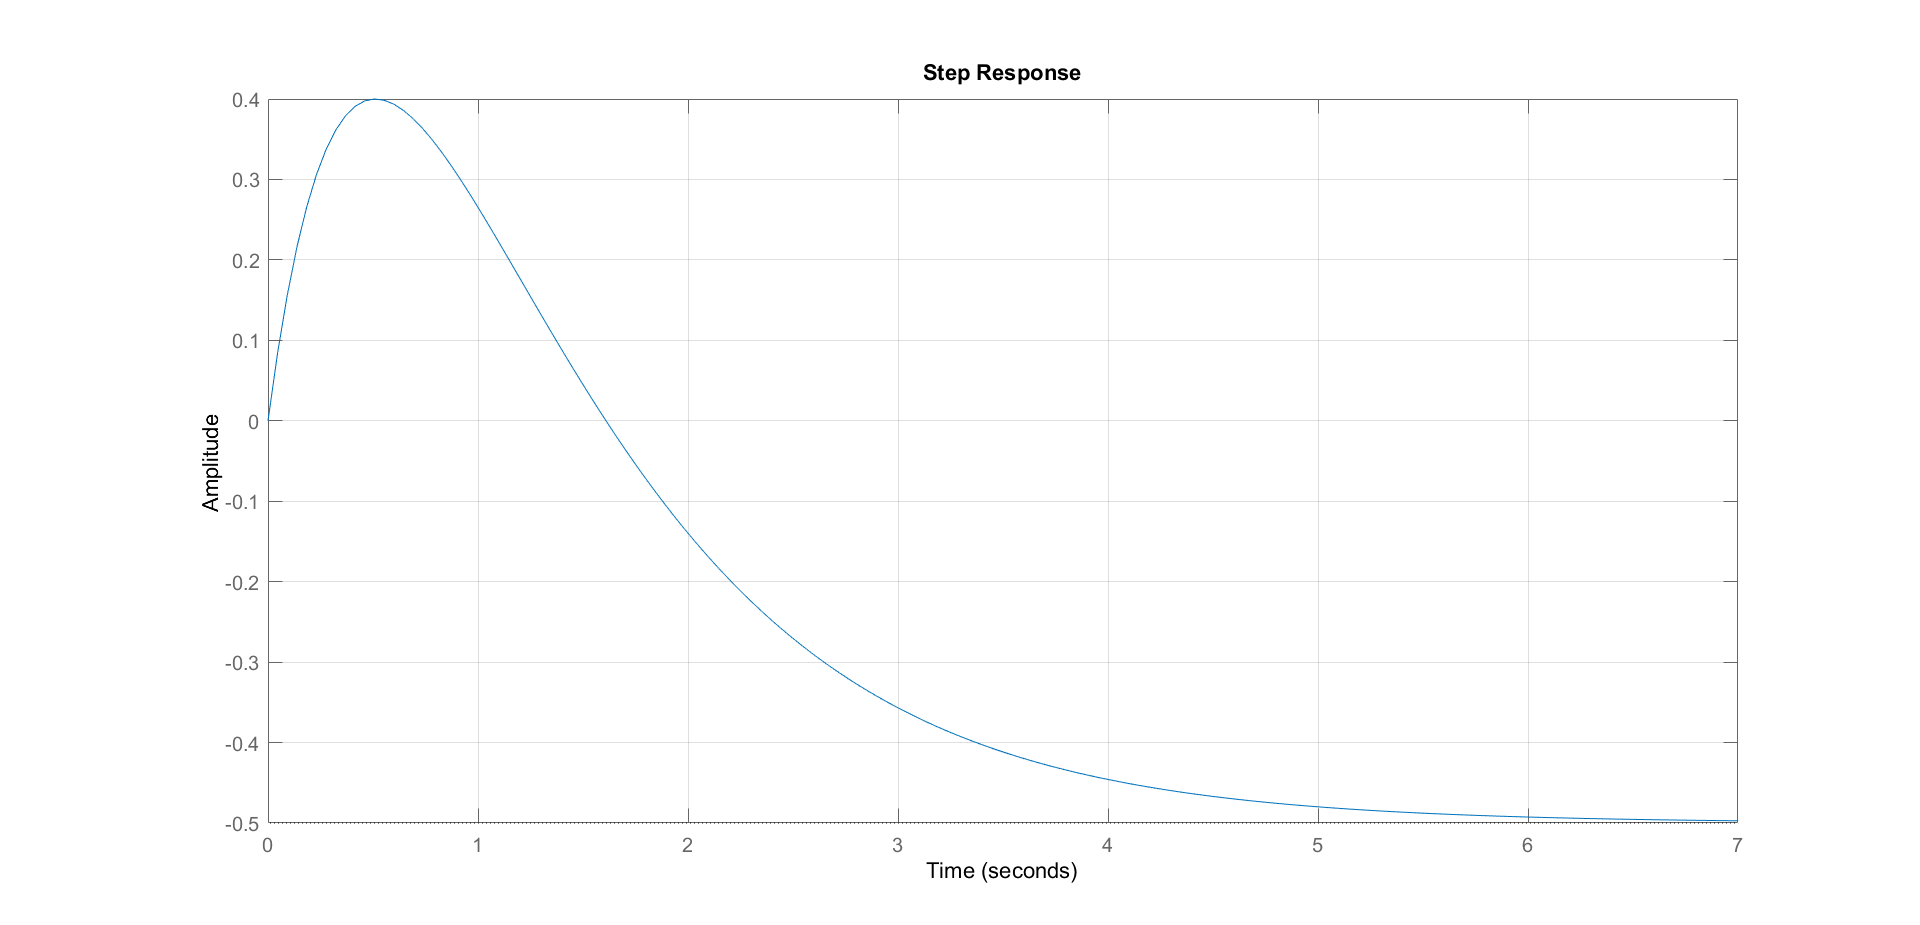
\includegraphics[width=\textwidth]{3_h_t.png}
    \caption{Переходная функция.}
    \label{fig:3_h_t.png}
\end{figure}

Найдем передаточную функцию, используя метод аппросимации Эйлера:
\[
    W_d(s) = W_c(\frac{s - 1}{h}) = \frac{2sh - h^2 - 2h}{s^2 + (3h - 2)s + 2h^2 - 3h + 1}
\]

Оценка на шаг дискретизации, при котором метод Эйлера дает устойчивую аппроксимацию:
\[
    h < \min_i \frac{|2 \Re \lambda_i(A)|}{|\lambda_i(A)|^2}
\]
\[
    \lambda_1 = -1, \ \lambda_2 = -2
\]
Тогда: 
\[
    q_1 = \frac{2}{1} = 2, \ q_2 = \frac{4}{4} = 1
\]
\[
    h < 1
\]

Проверим полученное значение, построив переходную функцию полученной дискретной системы для двух разных шагов дискретизации: в первом случае дискретная система должна быть устойчива, а во втором – неустойчива.

\begin{figure}[H]
    \centering
    \begin{subfigure}{0.49\textwidth}
        \centering
        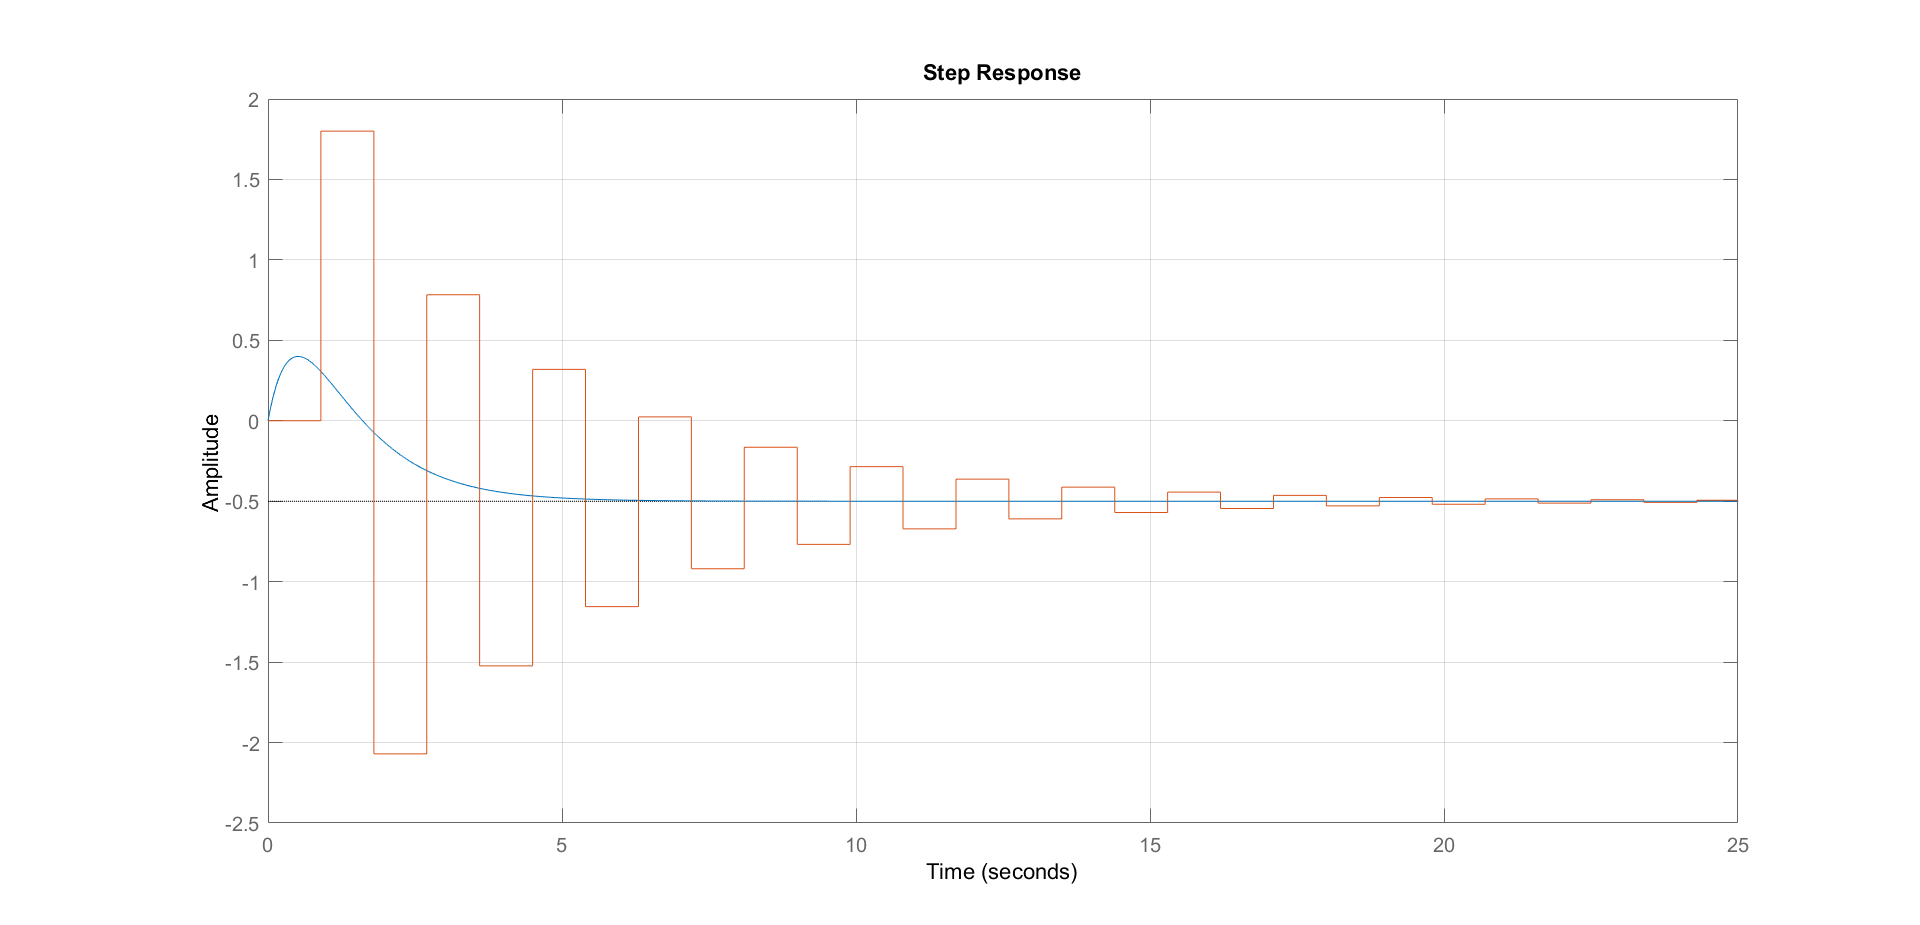
\includegraphics[width=\textwidth]{3_low_h.png}
        \caption{$h = 0.9$ - устойчивый случай}
         \label{fig:3_low_h.png}
     \end{subfigure}
     \hfill
     \begin{subfigure}{0.49\textwidth}
         \centering
         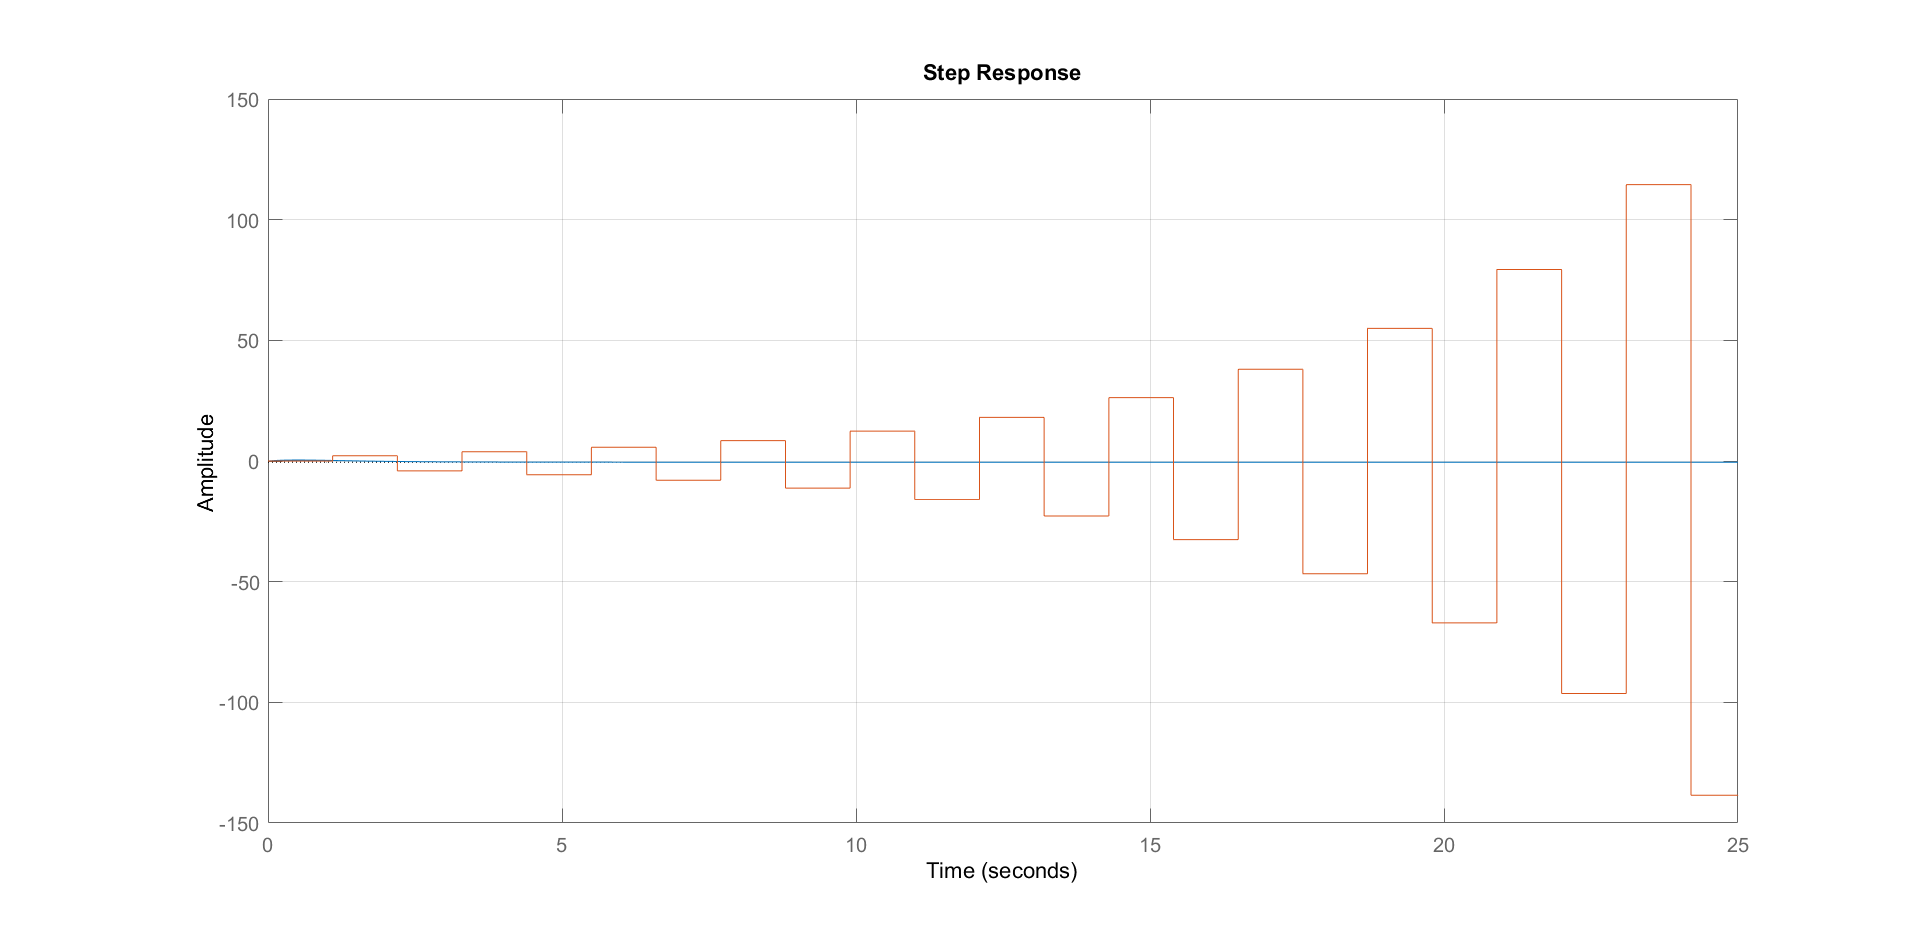
\includegraphics[width=\textwidth]{3_high_h.png}
         \caption{$h = 1.1$ - неустойчивый случай}
         \label{fig:3_high_h.png}
     \end{subfigure}
    \caption{Переходные функции дискретной и непрерывной систем.}
    \label{fig:two graphs}
\end{figure}

Найдем передаточную функцию дискретной системы, соответствующей исходной, по методу Тастина:
\[
    e^{Ah} \approx (I + \frac{Ah}{2})(I - \frac{Ah}{2})^{-1}
\]
\[
    W_d(s) = W_c(\frac{2s - 1}{hs + 1}) = \frac{s^2(4h - h^2) + s(4-4h) - 11.22}{s^2(2h^2 + 6h + 4) + s(h + 2)}
\]
Данная система устойчива при $\forall h > 0$.
\ \\
Построим переходную функцию полученной дискретной системы при $h = 1.1$:
\begin{figure}[H]
    \centering
    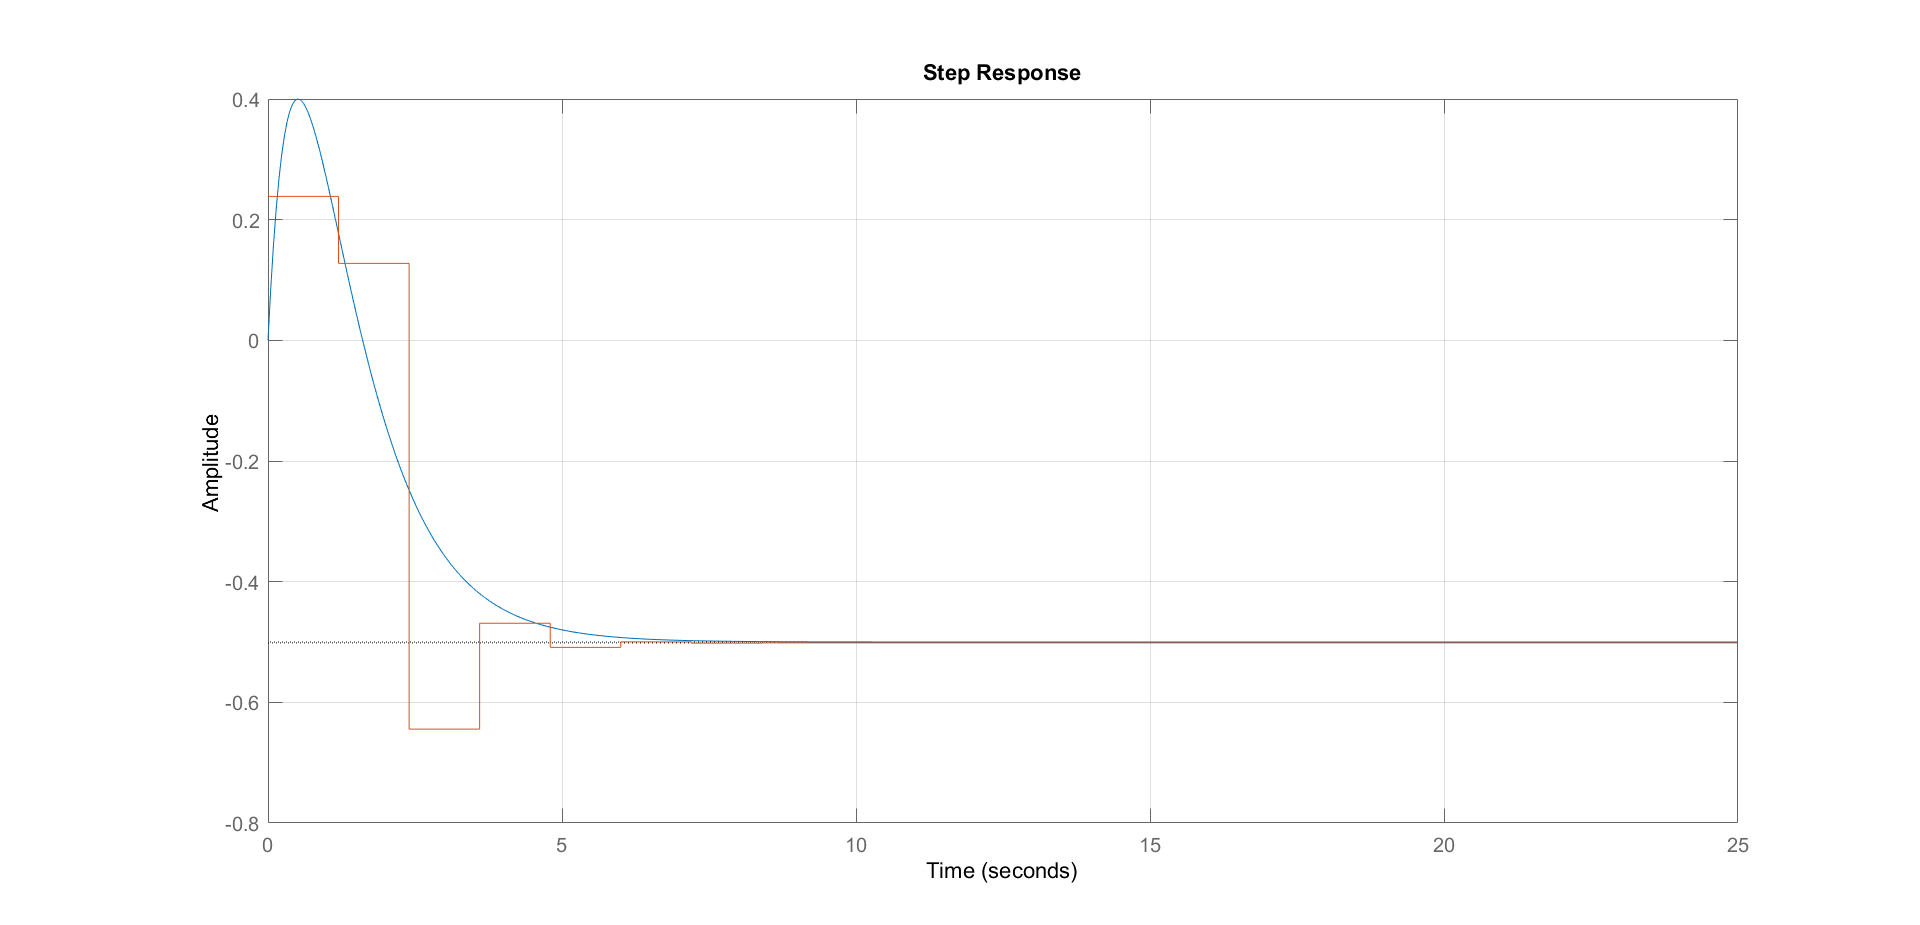
\includegraphics[width=\textwidth]{3_dustin.png}
    \caption{Переходные функции дискретной и непрерывной систем.}
    \label{fig:3_dustin.png}
\end{figure}

Переходная функция дискретной системы, полученной по методу Тастина, изображена выше. Как видно, при шаге дискретизации $h = 1.1$ метод Эйлера дает неустойчивую аппроксимацию, тогда как метод Тастина дает устойчивую.

\section*{Выводы}
В данной лабораторной работе была проделана работа по дискретизации непрерывных систем. В начале работы были проведены эквивалентные переходы между различными формами дискретных систем (такие же как и в случае непрерывных систем). \\
Во второй части работы требовалось получить дискретную систему различными способами: способом аппроксимации Эйлера и способом матричных дробей Паде (порядок (2, 2) - метод Тастина). \\ 
Метод Дастина сложен при вычислении, однако дает больший диапазон значения шага $h$ в сравнении с методом Эйлера.

\end{document}